\section{Derivation of the Wiener response}
\label{app:wiener}

We expand the linear-MMSE argument of Sec.~\ref{sec:gate}. Work in one
channel and assume wide-sense stationarity, so that convolution
diagonalizes in the Fourier basis and the mean-square error splits per
frequency.

\paragraph{Setup.} Under the mixture $x_t = a_t x_0 + b_t \varepsilon$ with
$\varepsilon$ white and independent of $x_0$, let $S_x(f)$ be the power
spectrum of $x_0$. For a linear filter $h_t$ with response $H_t(f)$,
Parseval's identity gives
\begin{equation}
  J_t(h_t) = \sum_f \Big(
  |H_t(f)|^2\big(a_t^2 S_x(f) + b_t^2\big)
  - 2\,\mathrm{Re}\big[H_t(f)\,a_t S_x(f)\big]
  + S_x(f)\Big).
  \label{eq:app-mse}
\end{equation}

\paragraph{Optimality by differentiation.} The summands decouple, so each
$H_t(f)$ solves a scalar problem. Differentiating with respect to
$\overline{H_t(f)}$ and setting to zero,
\begin{equation}
  H_t(f)\big(a_t^2 S_x(f) + b_t^2\big) - a_t S_x(f) = 0,
\end{equation}
which yields~\eqref{eq:wiener}. The second derivative
$a_t^2 S_x(f) + b_t^2 > 0$ confirms a minimum.

\paragraph{Power-law prior and spectral evolution.}
Natural images obey $S_x(f) \propto 1/|f|^p$ with $p \approx 2$.
Inserting this into~\eqref{eq:wiener}: at large $t$ (small $a_t$) the
denominator is noise-dominated except near $f = 0$, so $G_t$ is low-pass;
as $t \to 0$ ($a_t \to 1$) the passband widens toward high frequencies.
Fig.~\ref{fig:app-filters} plots the exact responses along the flow
schedule. This is the spectral evolution tracked by the filtered
distance of Sec.~\ref{sec:gate}, and the mean-gain
normalization~\eqref{eq:norm} makes those distances comparable across
$t$: the raw gains in Fig.~\ref{fig:app-filters}(a) differ by orders of
magnitude across $\sigma$, whereas the normalized responses in (b) share
a common scale and differ only in shape.

\begin{figure}[h]
  \centering
  
\includegraphics[width=0.95\linewidth]{figA_filters.pdf}
  \caption{Wiener filter responses along the flow schedule
  ($a_t = 1-\sigma$, $b_t = \sigma$, $S_x(f) = 1/|f|^p$, $p{=}2$ as used
  for FLUX; the video models use $p{=}3$ with the same qualitative
  shape). The formula is identical to SeaCache's; only the plotted
  schedule instance differs (flow, as used by our gate, vs.\ their
  DPM illustration). (a)~Raw response $G_t(f)$: low-pass early (large
  $\sigma$), widening as $\sigma \to 0$. (b)~Mean-normalized
  $G_t^{\mathrm{norm}}(f)$: comparable energy across timesteps, so
  accumulated distances are not dominated by gain drift. Computed from
  the closed form of~\eqref{eq:wiener}.}
  \label{fig:app-filters}
\end{figure}

%----------------------------------------------------------------
\section{Predictor hierarchy}
\label{app:hierarchy}

This section proves the three skip-length claims of
Secs.~\ref{sec:hierarchy}--\ref{sec:cheb}: copy-reuse is at most linear
in the skip length, degree-$P$ Taylor remainder is of order $P{+}1$, and
the Chebyshev truncation error does not depend on the skip length.
Throughout, $t_k$ is the last evaluated step and $t_j$ is the skipped
step at which the residual is reconstructed. The analysis is
channel-wise, as in the main text. The order-$P$ Taylor and Chebyshev
truncation statements are those of \citet[Thms.~3.1 and~3.2]{spectrum},
restated here for the residual trajectory $r$ in place of the hidden
state; the copy-reuse bound and the node-spacing refinement of the
discrete Taylor predictor are elementary.

\paragraph{Copy-reuse: linear bound.}
\label{app:reuse}
Copy-reuse sets $\hat{r}(t_j) = r(t_k)$. Assume $r$ is $L$-Lipschitz on
the sampling interval. Directly from the definition of Lipschitz
continuity,
\begin{equation}
  |r(t_j) - r(t_k)| \le L\,|t_j - t_k|,
\end{equation}
which is~\eqref{eq:reuse}. The bound is tight: $r(t) = Lt$ attains
equality for every skip. Lipschitz continuity is also necessary in the
worst case, since for a non-Lipschitz residual the ratio
$|r(t_j) - r(t_k)|/|t_j - t_k|$ is unbounded as the skip shrinks.
Copy-reuse uses no derivative
information, so additional smoothness ($r \in C^P$ for $P \ge 1$) cannot
improve this worst-case rate.

\paragraph{Taylor extrapolation: order-$(P{+}1)$ remainder.}
\label{app:taylor}
Assume $r \in C^{P+1}$. The degree-$P$ Taylor expansion of $r$ about
$t_k$ reads
\begin{equation}
  r(t_j)
  = \sum_{p=0}^{P} \frac{r^{(p)}(t_k)}{p!}\,(t_j-t_k)^p
  + R_P(t_j),
\end{equation}
with Lagrange remainder
\begin{equation}
  R_P(t_j)
  = \frac{r^{(P+1)}(\xi)}{(P{+}1)!}\,(t_j-t_k)^{P+1}
\end{equation}
for some $\xi$ between $t_k$ and $t_j$. Hence
$|R_P(t_j)| \le \frac{\|r^{(P+1)}\|_\infty}{(P{+}1)!}\,|t_j-t_k|^{P+1}$,
a $(P{+}1)$-order dependence on the skip length. This is the ideal
predictor: it uses the exact derivatives at $t_k$, which a
training-free cache never computes. In the discrete implementation the
derivatives $r^{(p)}(t_k)$ are replaced by backward differences
$\Delta^p r/(\Delta t)^p$ formed from $P{+}1$ neighboring evaluated
residuals $s_0 {=} t_k, s_1, \dots, s_P$, so the predictor is the
degree-$P$ interpolant $p_P$ through those nodes, with remainder
\begin{equation}
  r(t_j) - p_P(t_j)
  = \frac{r^{(P+1)}(\xi)}{(P{+}1)!}\prod_{q=0}^{P}(t_j - s_q)
  \label{eq:app-interp}
\end{equation}
for some $\xi$ in the convex hull of $\{t_j, s_0, \dots, s_P\}$. Only
the $q{=}0$ factor shrinks with the skip length
$\ell = |t_j - t_k|$; the remaining factors are fixed by the positions
of the earlier evaluated nodes. The $(P{+}1)$-order rate therefore
requires the node-spacing condition
$\max_q |t_j - s_q| \le C_{\mathrm{node}}\,\ell$, under which
$|r(t_j) - p_P(t_j)| \le C_{\mathrm{node}}^{P+1}
\|r^{(P+1)}\|_\infty \ell^{P+1}/(P{+}1)!$. The dynamic schedule does
not guarantee a uniform $C_{\mathrm{node}}$: with the earlier nodes
held fixed and $\ell \to 0$ the error is $O(\ell)$, not
$O(\ell^{P+1})$. The failure is sharp, not a loose estimate. Take
$P = 1$, $r(t) = t^2$, nodes $s_0 = t_k = 0$ and $s_1 = -H$ with
$H > 0$, and forecast point $t_j = \ell > 0$. The linear interpolant
through $(0,0)$ and $(-H,H^2)$ is $p_1(t) = -Ht$, so
$|r(\ell) - p_1(\ell)| = \ell(\ell + H)$ and
\begin{equation}
  \frac{|r(\ell) - p_1(\ell)|}{\ell^2} = 1 + \frac{H}{\ell},
  \label{eq:app-counterexample}
\end{equation}
which is unbounded as $H/\ell \to \infty$: no uniform constant over
arbitrary node configurations yields a bound of the form
$|r(t_j) - p_P(t_j)| \le C\,\ell^{P+1}$. Even uniform backward spacing
does not recover the ideal rate: for $t_j = t_k + \ell$ and
$s_q = t_k - qh$ with $h > 0$,
\begin{equation}
  \prod_{q=0}^{P}|t_j - s_q| = \prod_{q=0}^{P}(\ell + qh),
  \label{eq:app-uniform-product}
\end{equation}
a degree-$(P{+}1)$ polynomial in $\ell$ that coincides with
$\ell^{P+1}$ only in the limit $h/\ell \to 0$. In addition, the difference
operator amplifies observation noise by binomial coefficients of order
$2^P$. A higher $P$ therefore tightens the bound only for short skips
and becomes unstable as $|t_j-t_k|$ grows. The predictor also uses only
the $P{+}1$ most recent evaluations, discarding earlier trajectory
information.

\paragraph{Chebyshev truncation: skip-length-independent bound.}
\label{app:cheb}
Map the solver index to $\tau \in [-1,1]$ by an affine change of
variable, and write $r$ for the residual as a function of $\tau$. Let
$E_\rho$, $\rho > 1$, be the Bernstein ellipse with foci $\pm 1$ and
semi-axis sum $\rho$, and assume $r$ extends analytically to $E_\rho$
with $|r| \le B$ there. The Chebyshev coefficients then admit the
contour representation
$c_m = \frac{1}{\pi i}\oint_{E_\rho} r(z)\,T_m(z)^{-1}\,dz/z$ up to the
standard $m=0$ factor. On $E_\rho$ one has
$|T_m| \ge (\rho^m - \rho^{-m})/2$, which yields $|c_m| \le 2B\rho^{-m}$
for $m \ge 1$ and $|c_0| \le B$. Since $|T_m(\tau)| \le 1$ on $[-1,1]$,
truncating at degree $M$ leaves
\begin{equation}
  \|r - p_M^\star\|_\infty \le \sum_{m=M+1}^{\infty} 2B\rho^{-m}
  = \frac{2B}{\rho - 1}\,\rho^{-M},
\end{equation}
which is~\eqref{eq:cheb}. The right-hand side depends on $M$, $\rho$,
and $B$, but not on the evaluation point $\tau_j$. Consequently the
approximation-theoretic term is independent of the skip length
$|t_j-t_k|$. (The finite-sample ridge deviation from $p_M^\star$ is
controlled separately by Lemma~\ref{lem:ridge}.)

\paragraph{Node spacing versus design conditioning.}
The relative node-spacing condition above and the design-conditioning
quantity $\sigma_{\min}(\mathbf{\Phi})$ of Lemma~\ref{lem:ridge} are
distinct properties of the realized schedule: the former governs the
local interpolation remainder, the latter the stability of the fitted
Chebyshev coefficients, and neither implies the other. For one
direction, let the forecast distance $\ell > 0$ stay fixed while the
earlier nodes coalesce onto $t_k$; then
$\max_q|t_j - s_q|/\ell \to 1$, so the spacing condition holds with
$C_{\mathrm{node}} \to 1$, yet under the fixed affine normalization
the rows of $\mathbf{\Phi}$ become nearly identical and
$\sigma_{\min}(\mathbf{\Phi}) \to 0$ for any nonconstant basis.
Conversely, a fixed well-spread $K$-point design keeps
$\sigma_{\min}$ bounded away from zero while a forecast with
$\ell \to 0^+$ against a fixed distant node drives
$\max_q|t_j - s_q|/\ell \to \infty$. The ridge analysis of
Lemma~\ref{lem:ridge} is therefore not redundant alongside the
interpolation analysis: each controls a separate failure mode.

%----------------------------------------------------------------
\section{Proof of Lemma~\ref{lem:ridge} (ridge stability)}
\label{app:ridge}

The statement is Theorem~3.3 of \citet{spectrum}. We reproduce the
argument for the residual trajectory $r$ in place of the hidden state,
carrying the constants explicitly.

Fix one residual channel and drop the channel index, and take
$\lambda > 0$. Write the $K$
observations as $\mathbf{y} = \mathbf{\Phi}\mathbf{c}^\star + \mathbf{e}$,
where $\mathbf{c}^\star$ are the exact Chebyshev coefficients of
$p_M^\star$ and, by~\eqref{eq:cheb}, each entry of $\mathbf{e}$ satisfies
$|e_k| \le \varepsilon_M$, so $\|\mathbf{e}\|_2 \le \sqrt{K}\,\varepsilon_M$.
The ridge estimate is
$\hat{\mathbf{c}} = (\mathbf{\Phi}^\top\mathbf{\Phi} + \lambda I)^{-1}
\mathbf{\Phi}^\top \mathbf{y}$, hence
\begin{equation}
  \hat{\mathbf{c}} - \mathbf{c}^\star
  = (\mathbf{\Phi}^\top\mathbf{\Phi} + \lambda I)^{-1}\mathbf{\Phi}^\top \mathbf{e}
  - \lambda(\mathbf{\Phi}^\top\mathbf{\Phi} + \lambda I)^{-1}\mathbf{c}^\star.
  \label{eq:app-split}
\end{equation}
The forecast error at $\tau_j$ is the inner product of
$\hat{\mathbf{c}} - \mathbf{c}^\star$ with the basis row vector
$\boldsymbol{\phi}(\tau_j) = [T_0(\tau_j), \dots, T_M(\tau_j)]$, and
$|T_m| \le 1$ on $[-1,1]$ gives
$\|\boldsymbol{\phi}(\tau_j)\|_2 \le \sqrt{M{+}1\strut}$. Let
$\sigma_1 \ge \dots \ge \sigma_{M+1} = \sigma_{\min}$ be the singular
values of $\mathbf{\Phi} \in \mathbb{R}^{K \times (M+1)}$, with
$\sigma_{\min} = 0$ whenever $K < M{+}1$. We bound the two terms
of~\eqref{eq:app-split} in turn.

\paragraph{Variance term.} In the singular-value decomposition of
$\mathbf{\Phi}$,
\begin{equation}
  \|(\mathbf{\Phi}^\top\mathbf{\Phi} + \lambda I)^{-1}\mathbf{\Phi}^\top\|_2
  = \max_i \frac{\sigma_i}{\sigma_i^2 + \lambda}
  \le \frac{\sigma_1}{\sigma_{\min}^2 + \lambda},
\end{equation}
and every entry of $\mathbf{\Phi}$ is bounded by one, so
$\sigma_1 \le \|\mathbf{\Phi}\|_F \le \sqrt{(M{+}1)K}$. Combining this
with $\|\boldsymbol{\phi}(\tau_j)\|_2 \le \sqrt{M{+}1\strut}$ and
$\|\mathbf{e}\|_2 \le \sqrt{K}\,\varepsilon_M$,
\begin{equation}
  \bigl|\boldsymbol{\phi}(\tau_j)
  (\mathbf{\Phi}^\top\mathbf{\Phi} + \lambda I)^{-1}\mathbf{\Phi}^\top \mathbf{e}\bigr|
  \le \sqrt{M{+}1\strut}\cdot\frac{\sqrt{(M{+}1)K}}{\sigma_{\min}^2 + \lambda}
      \cdot\sqrt{K}\,\varepsilon_M
  = \frac{(M{+}1)K}{\sigma_{\min}^2 + \lambda}\,\varepsilon_M.
\end{equation}

\paragraph{Bias term.} The Chebyshev coefficients of a function
analytic on $E_\rho$ and bounded by $B$ there satisfy
$|c^\star_m| \le 2B\rho^{-m}$ (App.~\ref{app:cheb}), so
\begin{equation}
  \|\mathbf{c}^\star\|_2
  \le 2B\Bigl(\sum_{m \ge 0}\rho^{-2m}\Bigr)^{1/2}
  = \frac{2B}{\sqrt{1-\rho^{-2}}},
\end{equation}
a bound independent of $M$. Since the eigenvalues of
$(\mathbf{\Phi}^\top\mathbf{\Phi} + \lambda I)^{-1}$ are
$1/(\sigma_i^2 + \lambda)$, its spectral norm is
$1/(\sigma_{\min}^2 + \lambda)$, and therefore
\begin{equation}
  \bigl|\boldsymbol{\phi}(\tau_j)\,
  \lambda(\mathbf{\Phi}^\top\mathbf{\Phi} + \lambda I)^{-1}\mathbf{c}^\star\bigr|
  \le \frac{\lambda\sqrt{M{+}1\strut}}{\sigma_{\min}^2 + \lambda}
      \cdot\frac{2B}{\sqrt{1-\rho^{-2}}}.
\end{equation}

\paragraph{Combination.} Adding the two bounds gives
Lemma~\ref{lem:ridge}. Adding $\varepsilon_M$ once more,
by~\eqref{eq:cheb} and the triangle inequality, bounds the total error
$|r(\tau_j) - \hat{r}(\tau_j)|$ and recovers Theorem~3.3
of \citet{spectrum}. The two terms expose the trade-off: further
observations raise $\sigma_{\min}$ and keep the variance factor
bounded, while $\lambda$ guards the rank-deficient regime $K < M{+}1$
at the price of bias.

%----------------------------------------------------------------
\section{Residual-space error identity and conditioning}
\label{app:residual}

On a skipped step the block input $\mathbf{h}_{\mathrm{in}}$ is known
exactly from the current sampling state and the preceding computation,
so with $\mathbf{h}_{\mathrm{out}} = \mathbf{h}_{\mathrm{in}} + \mathbf{r}$,
\begin{equation}
  \hat{\mathbf{h}}_{\mathrm{out}} - \mathbf{h}_{\mathrm{out}}
  = \hat{\mathbf{r}} - \mathbf{r},
\end{equation}
i.e.\ state and residual forecasts share the same error for a fixed fit.
The fits differ in their regression target. Stacking the observed
input, output, and residual rows gives matrices satisfying the exact
identity $\mathbf{H}_{\mathrm{out}} = \mathbf{H}_{\mathrm{in}} +
\mathbf{R}$, where $\mathbf{H}_{\mathrm{in}}$ varies with the sampling
step and is not rank one, so no low-rank decomposition is assumed.
Each hidden-state observation carries the large input component, which
the sampler already knows exactly; fitting the full state therefore
inflates the regression target without adding anything that needs
predicting. The ridge map is linear in its target, so scaling the
target scales the fitted coefficients and the absolute shrinkage bias
while the shrinkage factor $\lambda/(\sigma_{\min}^2 + \lambda)$ is
unchanged (App.~\ref{app:ridge}): the ridge constants scale with the
target norm through $B$, which bounds the analytic continuation of the
fitted trajectory. Forecasting $\mathbf{R}$ directly keeps the target
small-normed and tightens every constant in proportion, a
target-scale advantage rather than a design-conditioning one --- all
fits share the same design matrix $\mathbf{\Phi}$ and hence identical
conditioning. The skipped-step update is $\mathbf{h} \gets
\mathbf{h} + \hat{\mathbf{r}}$.

%----------------------------------------------------------------
\section{Blend optimum and warm-up threshold}
\label{app:blend}

\paragraph{Blend weight.} With uncorrelated Taylor error (squared bias
$b_T^2$) and Chebyshev error (variance $\sigma_C^2$), the blended risk is
$R(w) = (1-w)^2 b_T^2 + w^2\sigma_C^2$. Setting $R'(w) = 0$ gives
$w^\star = b_T^2/(b_T^2 + \sigma_C^2)$. Early in sampling both the drift
and the fit variance are large; late in sampling both shrink as the
trajectory settles and $K$ grows (Appendix~\ref{app:ridge}).
Measured trajectories keep the two terms within a factor of two of each
other, which places $w^\star$ near $1/2$ throughout and motivates the
fixed $w = 0.5$.

\paragraph{Warm-up.} With $n$ observations and $M{+}1$ bases, $n < M{+}1$
leaves~\eqref{eq:ridge} rank-deficient: $\sigma_{\min}(\mathbf{\Phi}) =
0$, the observations cannot identify all coefficient directions, and the
fit is dominated by the prior (the bias term of
Appendix~\ref{app:ridge} governs). The first-order discrete Taylor step is
exact on the last two observations by construction and therefore
strictly dominates in this regime. Blending from $n \ge 4$ onward (the
$M = 4$ fit being determined in practice) is thus the degrees-of-freedom
crossover rather than a tuned choice.

%----------------------------------------------------------------
\section{Refresh-ratio analysis}
\label{app:refresh}
Refresh histograms concentrate compute early along the trajectory, in
accordance with the spectral prior of~\eqref{eq:wiener}: evaluations are
dense while $G_t$ is narrow (content forming) and sparse as the passband
widens. PSNR-versus-refresh curves for ReSPect follow the full-compute
reference monotonically at both $\delta$ settings, with the gap to
copy-reuse widening at lower refresh ratios, precisely where the reuse
bound~\eqref{eq:reuse} loosens and the uniform bound~\eqref{eq:cheb}
remains tight, as anticipated in Sec.~\ref{sec:t2i}.

\begin{figure}[h]
  \centering
  
\includegraphics[width=0.95\linewidth]{figA_skip.pdf}
  \caption{Compute concentrates early; quality tracks full compute.
  Left: per-prompt skip-rate histograms (Wan). Right: per-prompt PSNR
  vs skip rate over full VBench-946.}
  \label{fig:app-refresh}
\end{figure}

\begin{figure}[h]
  \centering
  
\includegraphics[width=0.95\linewidth]{figA_ssim_lpips.pdf}
  \caption{Per-prompt SSIM/LPIPS clouds at each config's TFLOPs.
  Top: FLUX DrawBench-200. Bottom: Wan VBench-946 .}
  \label{fig:app-clouds}
\end{figure}

%----------------------------------------------------------------
\section{Implementation details}
\label{app:impl}

\paragraph{Forecaster.} $M{=}4$ Chebyshev bases, window $K{=}100$,
$\lambda{=}0.1$, blend $w{=}0.5$, first-order discrete Taylor,
Taylor-only warm-up until $n \ge 4$ observations. Time is mapped to
$\tau \in [-1,1]$ over the fixed range $[0, 50]$ (buffer min/max is
\emph{not} used). One forecaster per sample; coefficient state is a single
$(M{+}1)\times F$ matrix plus $K$ cached residuals.

\paragraph{Complexity.} Fitting is $\mathcal{O}(K(M{+}1)F)$ with
$M \ll K \ll F$ (the $(M{+}1)^3$ Cholesky term is negligible);
prediction is $\mathcal{O}((M{+}1)F)$; memory is
$\mathcal{O}((M{+}1)F + KF)$. Measured overhead is ${\sim}0.09$\,s/image
on FLUX. First and last steps always compute; CFG call streams are
demuxed by timestep equality.

\paragraph{Hardware and seeds.} FLUX.1-dev, DrawBench (200 prompts),
$1024{\times}1024$, 50 steps, guidance 3.5, bf16, seeds $0{+}i$.
Video: VBench prompts, 480p, 65 frames, 50 steps. All latencies are
wall-clock on a single NVIDIA B200; all quality claims are at matched NFE.

%----------------------------------------------------------------
\paragraph{Cost of the forecaster.} A latency column combines the
effects of schedule and reconstructor, since two methods at the same budget
may skip at different steps. Running both reconstructors in one harness
at the same $\delta$, which fixes the schedule and varies only what is
written on a skipped step, yields identical realized NFE: the gate reads
the modulated block input, so replacing copy-reuse with a forecast does
not alter where it fires. The forecast adds $1.7$--$4.3\%$ wall-clock
over copy-reuse (Tab.~\ref{tab:overhead}).

\begin{table}[h]
  \centering
  \caption{Cost of the reconstructor at fixed schedule. Both columns of each
  row use the same gate and the same $\delta$ in the same harness on one
  B200; only the skipped-step reconstruction differs. NFE is identical
  within every pair.}
  \label{tab:overhead}
  \vspace{0.1cm}
  {\small\setlength{\tabcolsep}{5pt}
  \begin{tabular}{llcccc}
    \toprule
    Model & $\delta$ & NFE & Copy-reuse (s) & Forecast (s) & $\Delta$ \\
    \midrule
    FLUX.1-dev   & 0.3  & 21 & 2.38  & 2.47  & $+3.8\%$ \\
    FLUX.1-dev   & 0.6  & 13 & 1.55  & 1.61  & $+3.9\%$ \\
    Wan2.1-1.3B  & 0.17 & 46 & 14.31 & 14.80 & $+3.4\%$ \\
    Wan2.1-1.3B  & 0.31 & 32 & 10.49 & 10.94 & $+4.3\%$ \\
    HunyuanVideo & 0.27 & 24 & 39.20 & 39.86 & $+1.7\%$ \\
    HunyuanVideo & 0.48 & 16 & 27.38 & 27.90 & $+1.9\%$ \\
    \bottomrule
  \end{tabular}}
\end{table}

\paragraph{ReSPect vs.\ SeaCache at matched schedules.}
We further compare ReSPect against SeaCache~\citep{seacache} copy-reuse
under matched schedules, tuning $\delta$ to equalize NFE. Both arms run
in our own harness: the gate is unchanged, so the two methods realize
(near-)identical NFE and only the skipped-step reconstruction differs.
Tab.~\ref{tab:abl-sea} reports full-reference quality against the
uncached outputs. The forecast wins on PSNR, SSIM, and LPIPS at every
setting with a matched pair: $+0.79$\,dB on FLUX $\delta{=}0.37$
($n{=}200$), $+0.49$\,dB on FLUX $\delta{=}0.6$ ($n{=}20$), and
$+0.93$\,dB on Wan $\delta{=}0.31$ ($n{=}20$), with LPIPS down $18\%$
where measured. We attribute this to the residual forecast tracking
the trajectory between evaluations, whereas copy-reuse holds the last
observed residual fixed.

\begin{table}[h]
  \centering
  \caption{ReSPect vs.\ SeaCache copy-reuse at matched schedules: same
  $\delta$, same prompts, (near-)identical NFE; only the skipped-step
  reconstruction differs. LPIPS was not measured on the 20-prompt
  subsets (---). The FLUX $\delta{=}0.37$ pair is full DrawBench-200;
  the $\delta{=}0.6$ and Wan pairs are fixed 20-prompt subsets.}
  \label{tab:abl-sea}
  \vspace{0.1cm}
  {\scriptsize\setlength{\tabcolsep}{4pt}
  \begin{tabular}{llcccc}
    \toprule
    Setting & Method & NFE & PSNR$\uparrow$ & SSIM$\uparrow$  \\
    \midrule
    FLUX $\delta{=}0.37$ & SeaCache & 18.1 & 25.45 & 0.880  \\
    ($n{=}200$) & \textbf{ReSPect} & \textbf{18.1} & \textbf{26.24} & \textbf{0.895}  \\
    \midrule
    FLUX $\delta{=}0.6$ & SeaCache & 13.0 & 23.08 & 0.848  \\
    ($n{=}20$) & \textbf{ReSPect} & \textbf{13.0} & \textbf{23.57} & \textbf{0.852} \\
    \midrule
    Wan $\delta{=}0.31$ & SeaCache & 32.4 & 28.80 & 0.904  \\
    ($n{=}20$) & \textbf{ReSPect} & \textbf{32.3} & \textbf{29.73} & \textbf{0.917} &  \\
    \bottomrule
  \end{tabular}}
\end{table}

\section{Reconstructor ablations against copy-reuse}
\label{app:abl-reuse}

All arms share one base run, so every $\Delta$dB value below is paired
against the same copy-reuse baseline (Fig.~\ref{fig:ablation}), run at
the aggressive budgets (FLUX $\delta{=}0.6$, Wan $\delta{=}0.31$) on
fixed 20-prompt subsets.

\paragraph{Blend weight $w$.}
Pure Taylor ($w{=}0$) is strong wherever neighboring evaluations carry
the signal: $+2.30$\,dB on Wan and $+0.50$\,dB on FLUX. Pure Chebyshev
($w{=}1$) fails precisely where the fit is least determined:
$-1.68$\,dB on Wan, with its long skip runs, and $+0.09$\,dB
($\approx$ copy-reuse) on FLUX. The fixed $w{=}0.5$ remains at or above
copy-reuse on either model ($+0.49$/$+0.93$\,dB); it is a robust
compromise, and the setting used in the main tables, rather than a
per-subset optimum.

\paragraph{Warm-up threshold.}
Blending before the fit is determined ($n < M{+}1$) lets the penalty
dominate the data. A warm-up of 8 attains the largest FLUX gain
($+0.68$\,dB) but lies within noise of the default blend; longer
Taylor-only spans (12--24) never accumulate enough observations to
blend at this budget and coincide with pure Taylor ($+0.50$\,dB).
Extending the warm-up is therefore without penalty, and the polynomial term
engages only once the fit is determined.

\paragraph{Window $K$.}
$K{=}32$ matches $K{=}100$ to three decimals ($+0.491$ vs.\
$+0.491$\,dB): per-prompt buffers rarely exceed ${\sim}40$
observations, so the $\sigma_{\min}$ gains of Lemma~\ref{lem:ridge}
have saturated early and $K{=}100$ is a conservative default rather than a
tuned choice.

\begin{figure}[h]
  \centering
  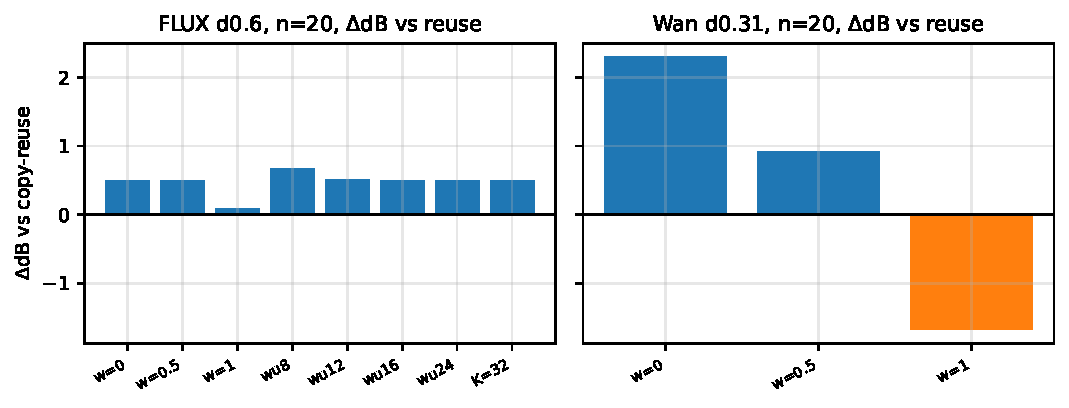
\includegraphics[width=0.9\linewidth]{figs/fig_ablation.pdf}
  \caption{Ablations ($\Delta$dB against copy-reuse, paired on one
  shared base run per panel). Left: FLUX $\delta{=}0.6$, $n{=}20$.
  Right: Wan $\delta{=}0.31$, $n{=}20$. Pure Taylor dominates on Wan
  while the blend remains at or above copy-reuse; pure Chebyshev fails on
  long skip runs; warm-ups of 12 and above never engage the blend; the
  window $K$ has saturated.}
  \label{fig:ablation}
\end{figure}

\section{Additional qualitative results}
\label{app:qual}

\begin{figure}[h]
  \centering
  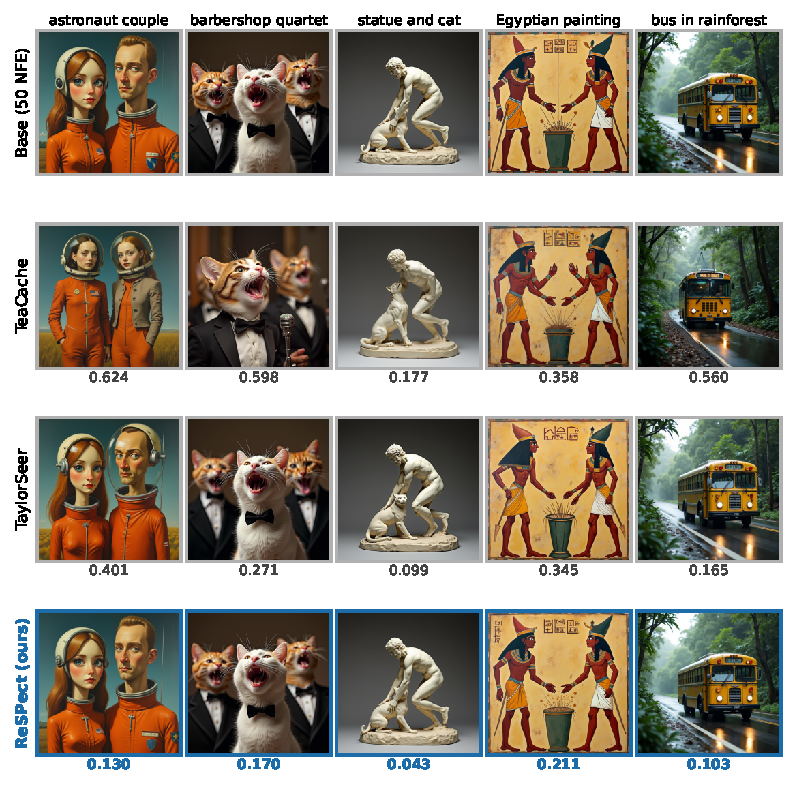
\includegraphics[width=\linewidth]{figs/fig_qual_flux.pdf}
  \caption{FLUX.1-dev at the aggressive budget, all methods run in our
  harness. ReSPect at $\delta{=}0.6$; TaylorSeer ($\mathcal{S}{=}5$) and
  TeaCache ($\delta{=}0.6$) use equal or more compute. LPIPS against the
  base image is printed under each panel. Over 20 DrawBench prompts
  ReSPect attains the lowest LPIPS on 19 (mean $0.183$ vs.\ $0.256$ and
  $0.407$).}
  \label{fig:qual}
\end{figure}

\begin{figure}[h]
  \centering
  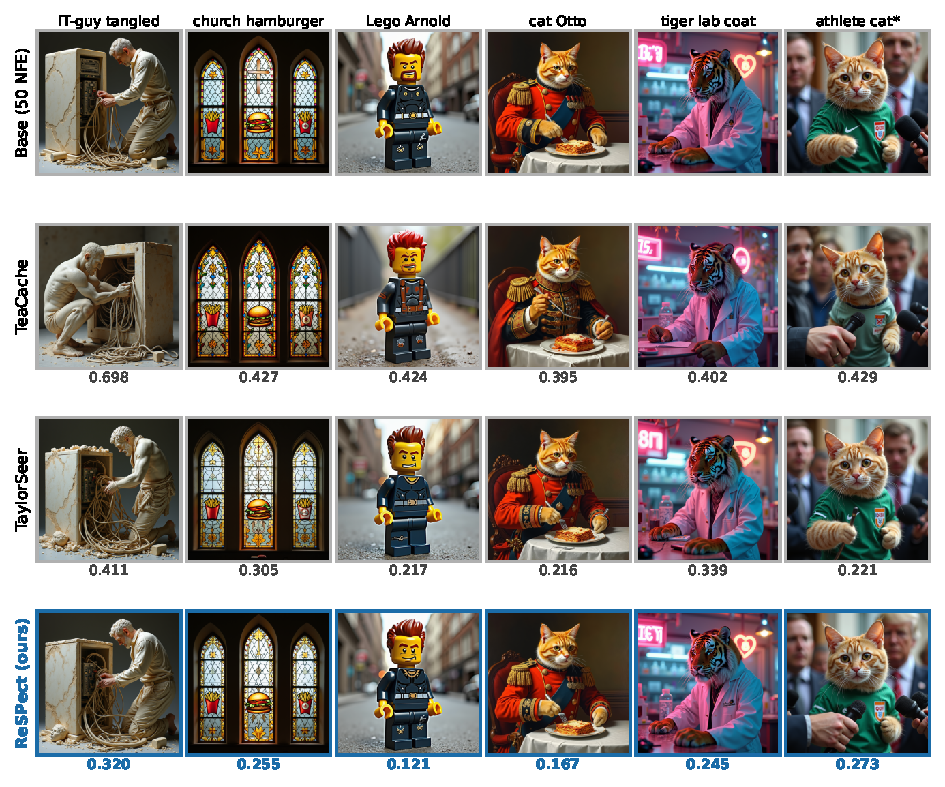
\includegraphics[width=\linewidth]{figs/fig_qual_flux_b.pdf}
  \caption{Six further DrawBench prompts at the same aggressive budget
  and harness as Fig.~\ref{fig:qual} (ReSPect $\delta{=}0.6$;
  TaylorSeer $\mathcal{S}{=}5$; TeaCache $\delta{=}0.6$). ReSPect is
  closest to the base on five of six; ``athlete cat*'' is the single
  prompt of the twenty where TaylorSeer attains the lower LPIPS
  ($0.221$ vs.\ $0.273$), shown here for completeness.}
  \label{fig:qual-b}
\end{figure}

All clips below are generated in our harness on one B200. ReSPect runs
at $\delta{=}0.31$ (Wan, 32 forward passes) and $\delta{=}0.48$
(Hunyuan, 16); TeaCache and TaylorSeer run at their published operating
points and use more compute . The two
sentence prompts are (retriever) ``A golden retriever running along a
sandy beach at sunset, waves rolling in behind it'' and (balloon) ``A
red hot air balloon drifting slowly over green rolling hills under a
clear blue sky''; both are also printed in the title of each strip
figure. Per-frame PSNR against the base frame is printed under each
panel. Averaged over all 65 frames, ReSPect leads on every clip:
Wan balloon $34.87$ vs.\ $31.29$ / $17.60$; Wan retriever $30.96$ vs.\
$27.07$ / $17.91$; Hunyuan balloon $37.41$ vs.\ $25.80$ / $21.52$;
Hunyuan retriever $26.04$ vs.\ $16.32$ / $15.24$
(TeaCache / TaylorSeer). The retriever prompt is a difficult motion
case in which all caches degrade while the ordering is preserved.
Tab.~\ref{tab:app-qual} gives the full per-prompt comparison with SSIM
and LPIPS (frame-averaged against the uncached same-seed reference).

\begin{table}[h]
  \centering
  \caption{Per-prompt qualitative-clip comparison: frame-averaged PSNR,
  SSIM, and LPIPS against the uncached same-seed reference over all 65
  frames. NFE is forward passes per clip (Wan base 100, Hunyuan base
  50). ReSPect uses the least compute and leads on every clip and
  metric.}
  \label{tab:app-qual}
  \vspace{0.1cm}
  {\scriptsize\setlength{\tabcolsep}{3pt}
  \begin{tabular}{llcccc}
    \toprule
    Clip & Method & PSNR$\uparrow$ & SSIM$\uparrow$ & LPIPS$\downarrow$ & NFE \\
    \midrule
    Wan retriever & TeaCache & 27.07 & 0.892 & 0.109 & 38 \\
    & TaylorSeer & 17.91 & 0.656 & 0.384 & 36 \\
    & \textbf{ReSPect} & \textbf{30.96} & \textbf{0.937} & \textbf{0.066} & \textbf{32} \\
    \midrule
    Wan balloon & TeaCache & 31.29 & 0.918 & 0.064 & 38 \\
    & TaylorSeer & 17.60 & 0.568 & 0.321 & 36 \\
    & \textbf{ReSPect} & \textbf{34.87} & \textbf{0.950} & \textbf{0.031} & \textbf{32} \\
    \midrule
    Hunyuan retriever & TeaCache & 16.32 & 0.669 & 0.322 & 18 \\
    & TaylorSeer & 15.24 & 0.643 & 0.379 & 18 \\
    & \textbf{ReSPect} & \textbf{26.04} & \textbf{0.878} & \textbf{0.089} & \textbf{16} \\
    \midrule
    Hunyuan balloon & TeaCache & 25.80 & 0.914 & 0.046 & 18 \\
    & TaylorSeer & 21.52 & 0.903 & 0.117 & 18 \\
    & \textbf{ReSPect} & \textbf{37.41} & \textbf{0.980} & \textbf{0.005} & \textbf{16} \\
    \bottomrule
  \end{tabular}}
\end{table}

\begin{figure}[h]
  \centering
  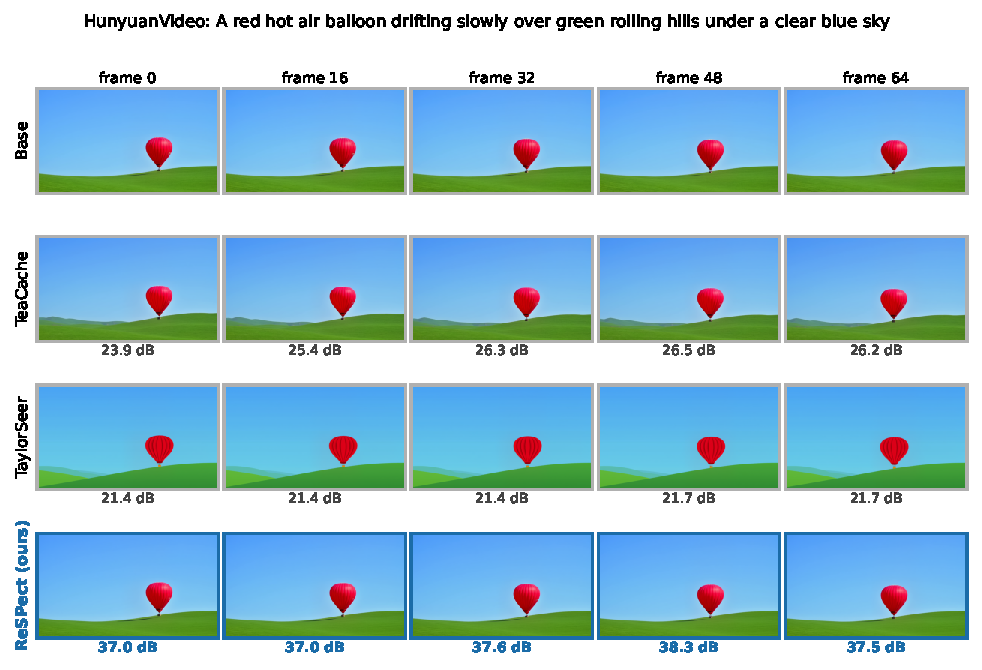
\includegraphics[width=\linewidth]{figs/fig_seq_hunyuan_p1.pdf}
  \caption{HunyuanVideo, balloon clip, $\delta{=}0.48$ (16 NFE).
  TaylorSeer renders a different scene entirely and retains it for the
  whole clip; averaged over all 65 frames, ReSPect scores $37.41$\,dB
  against $25.80$ (TeaCache) and $21.52$ (TaylorSeer).}
  \label{fig:app-qual-hun1}
\end{figure}

\begin{figure}[h]
  \centering
  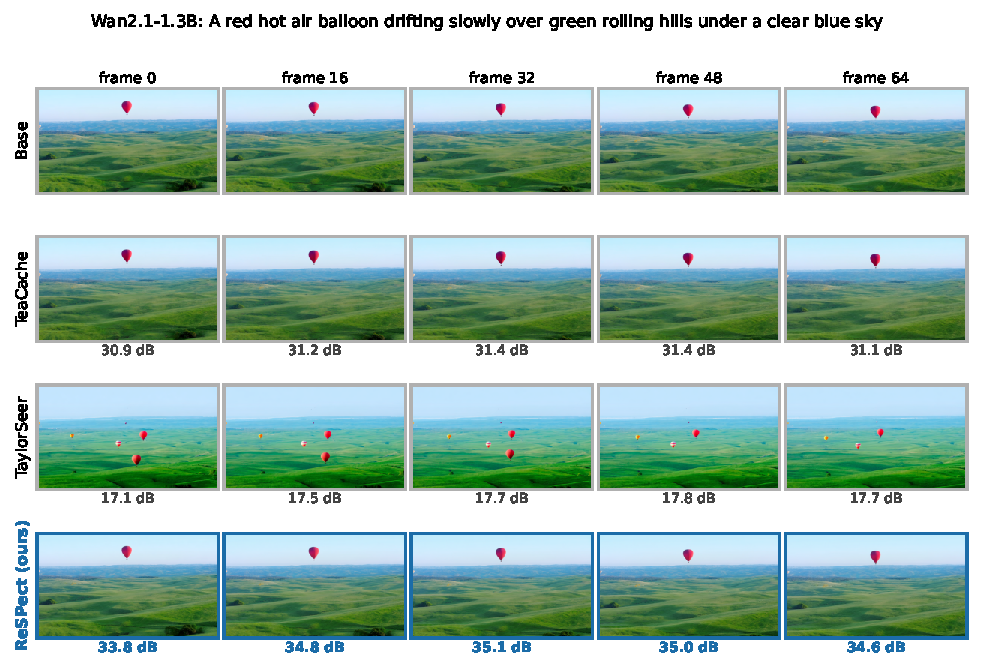
\includegraphics[width=\linewidth]{figs/fig_seq_wan_p1.pdf}
  \caption{Wan2.1, balloon clip, $\delta{=}0.31$ (32 NFE).
  TaylorSeer hallucinates three additional balloons
  and retains them for the whole clip.}
  \label{fig:app-qual}
\end{figure}

\begin{figure}[h]
  \centering
  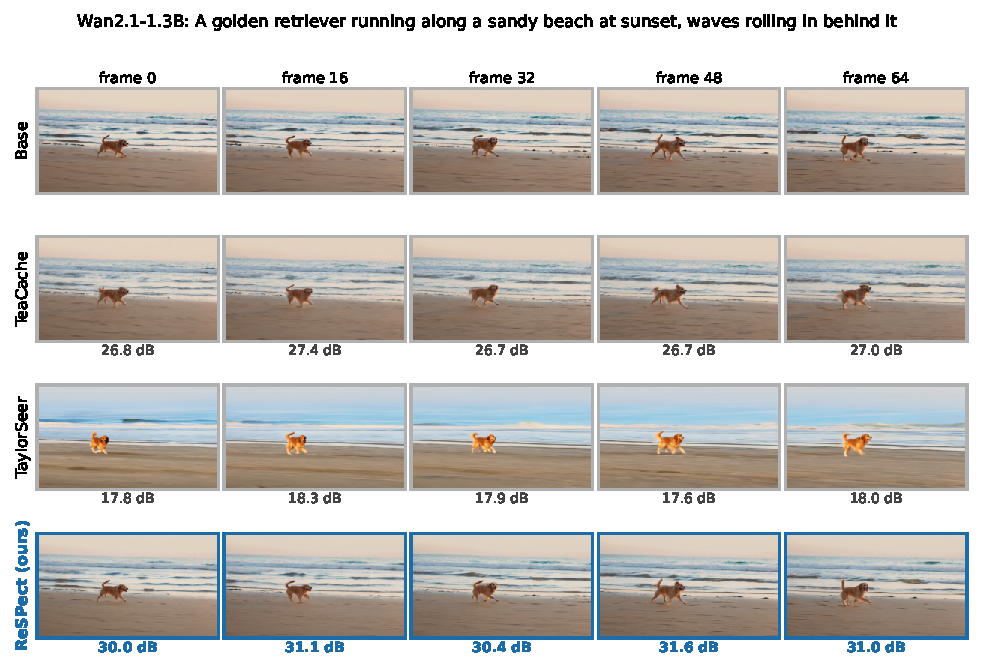
\includegraphics[width=\linewidth]{figs/fig_seq_wan_p0.pdf}
  \caption{Wan2.1, retriever clip, $\delta{=}0.31$ (32 NFE): a difficult
  motion prompt. All methods lie closer to the base here; the forecast
  still gains $+3.9$\,dB over the next baseline, whereas the
  interval-based and raw-distance schedules lose $4$--$13$\,dB.}
  \label{fig:app-qual-wan0}
\end{figure}

\begin{figure}[h]
  \centering
  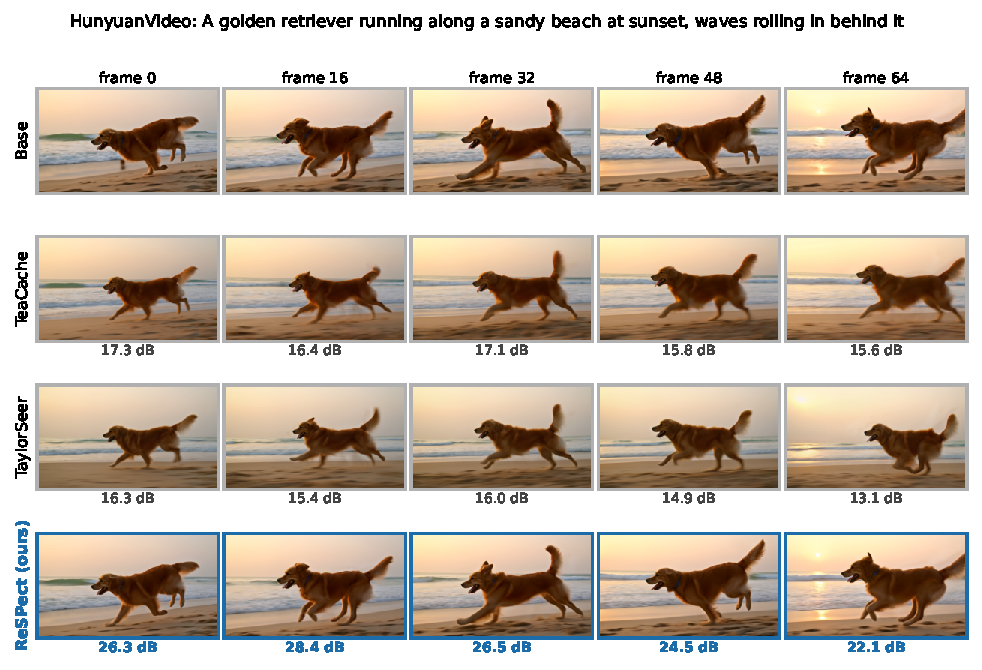
\includegraphics[width=\linewidth]{figs/fig_seq_hunyuan_p0.pdf}
  \caption{HunyuanVideo, retriever clip, $\delta{=}0.48$ (16 NFE).}
  \label{fig:app-qual-hun0}
\end{figure}

